\documentclass{article}

\usepackage[backend=biber, style=authortitle-icomp]{biblatex}
\addbibresource{uni.bib}
\usepackage{graphicx}
\usepackage{blindtext}
\usepackage{wrapfig}

\author{Chau Dinh}
\title{An Introduction to Labels, Refs, and Lists in {\LaTeX} }

\begin{document}

\maketitle

\section{Introduction}

So in this section \ref{list}, I will talk about lists in {\LaTeX}

Note we talk about toilet paper, which is number \ref{toil}.

Please refer to Figure \ref{latexpic}

\section{Lists\label{list}}

\begin{enumerate}
\item Bread
\item Toilet paper\label{toil}
\end{enumerate}

An unordered list:

\begin{itemize}
\item Corn
    \begin{itemize}
    \item red
    \item black
    \end{itemize}
\item Maize
\item a lamp
\end{itemize}

\section{Bibliography Management}

As \textcite{test} says, there is no reason to use {\LaTeX} for bibliography hahaahah.

\printbibliography

\section{Images}

Here is a new document

\begin{center}
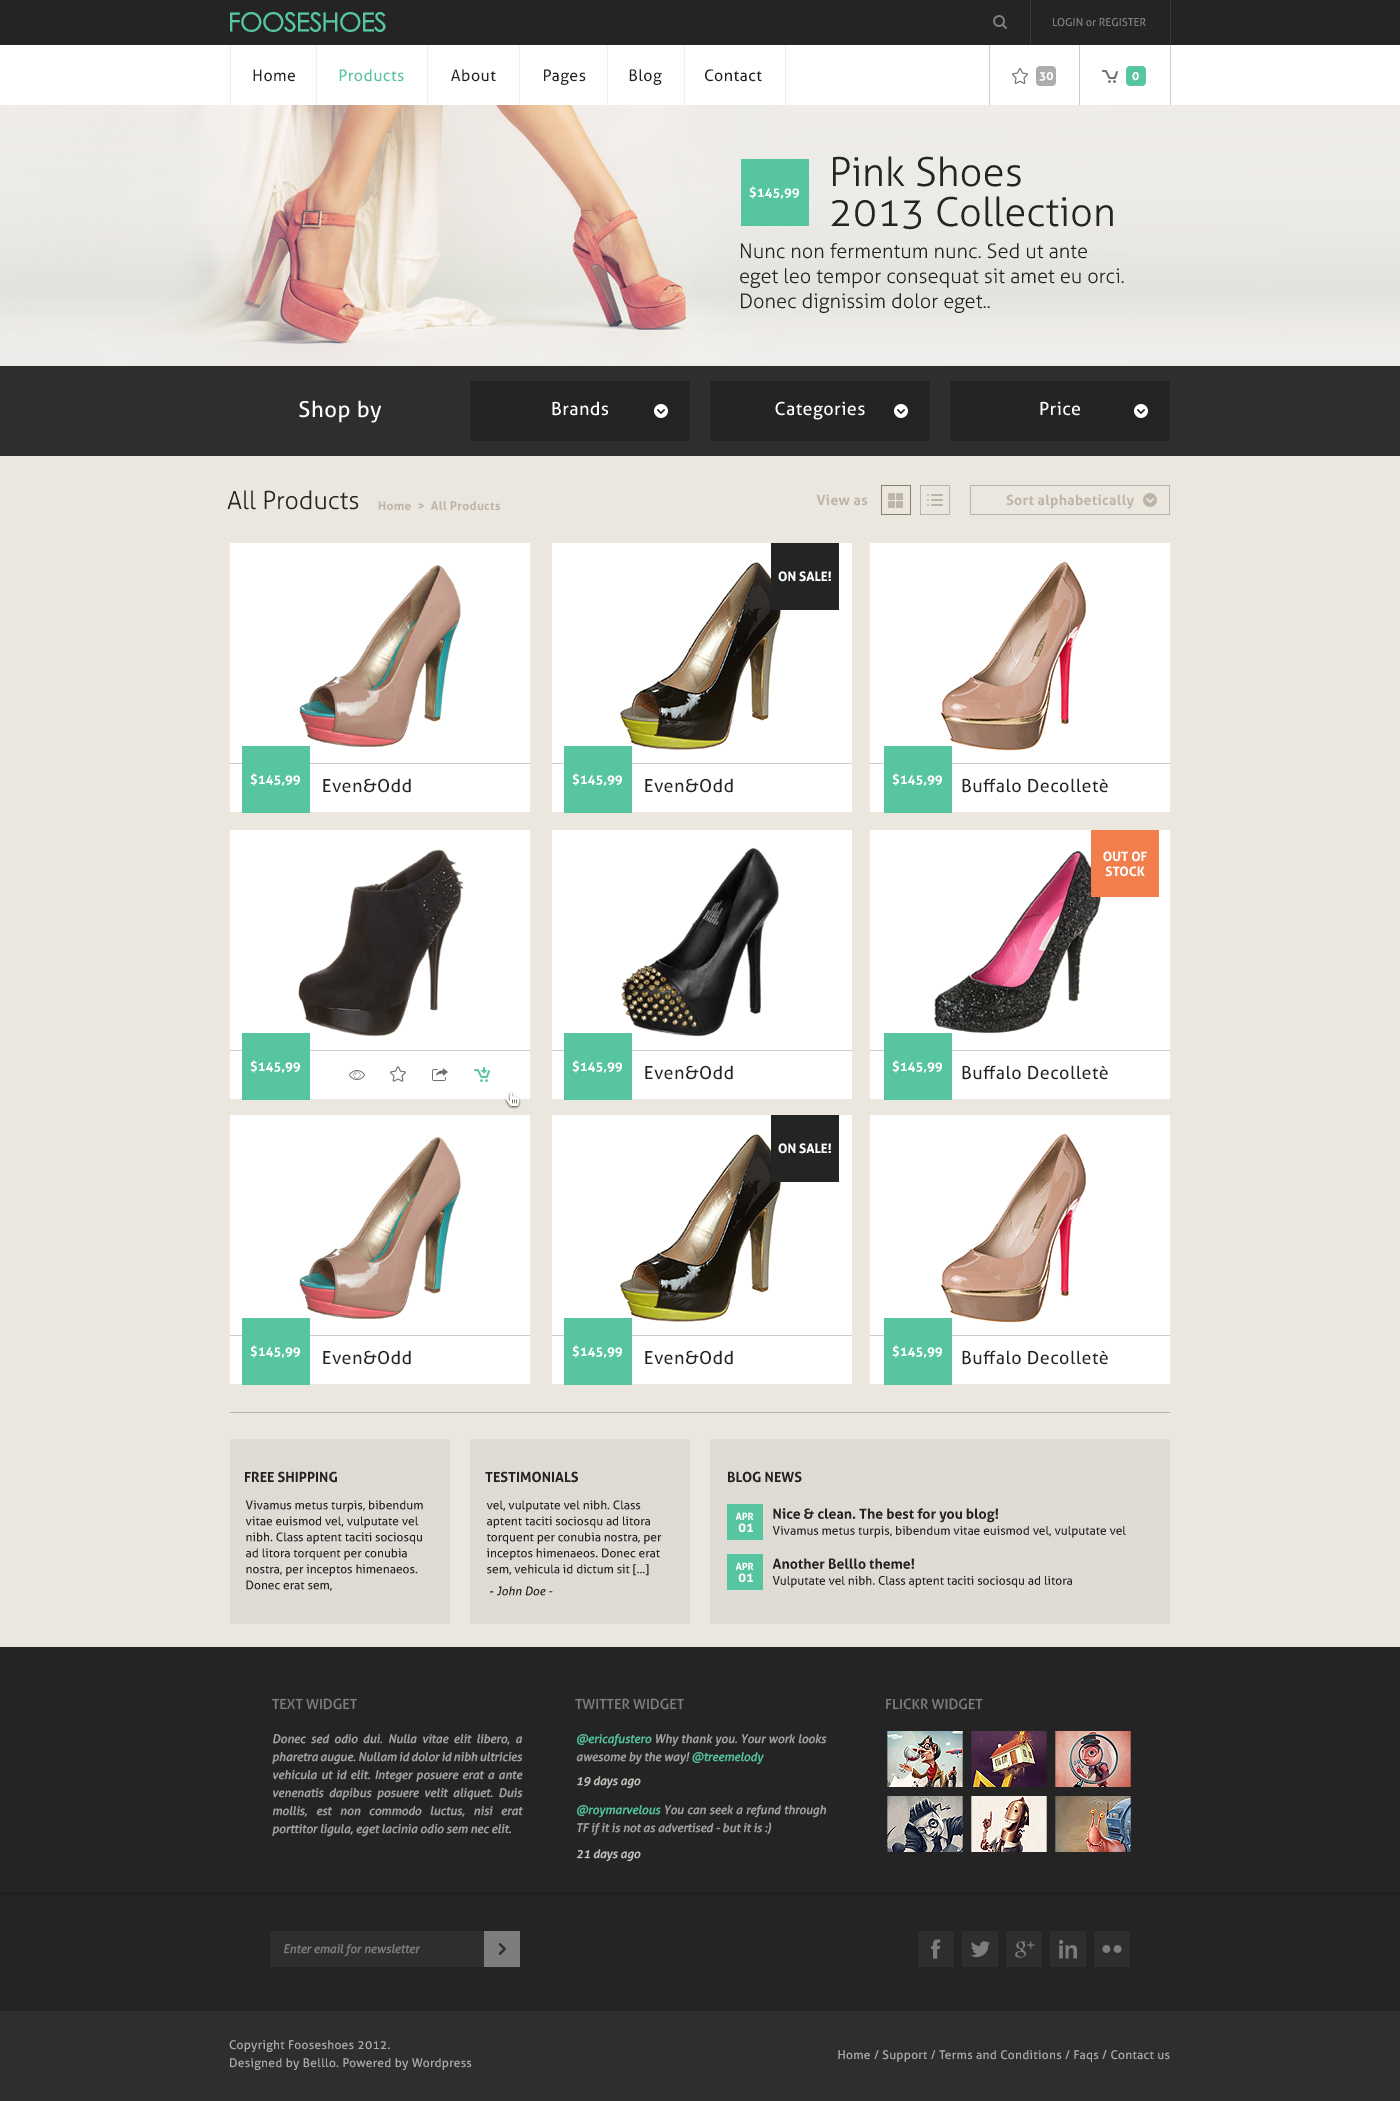
\includegraphics[width=0.7\textwidth]{demo.jpg}
\end{center}

\blindtext

\blindtext

\begin{figure}[h]
\centering 
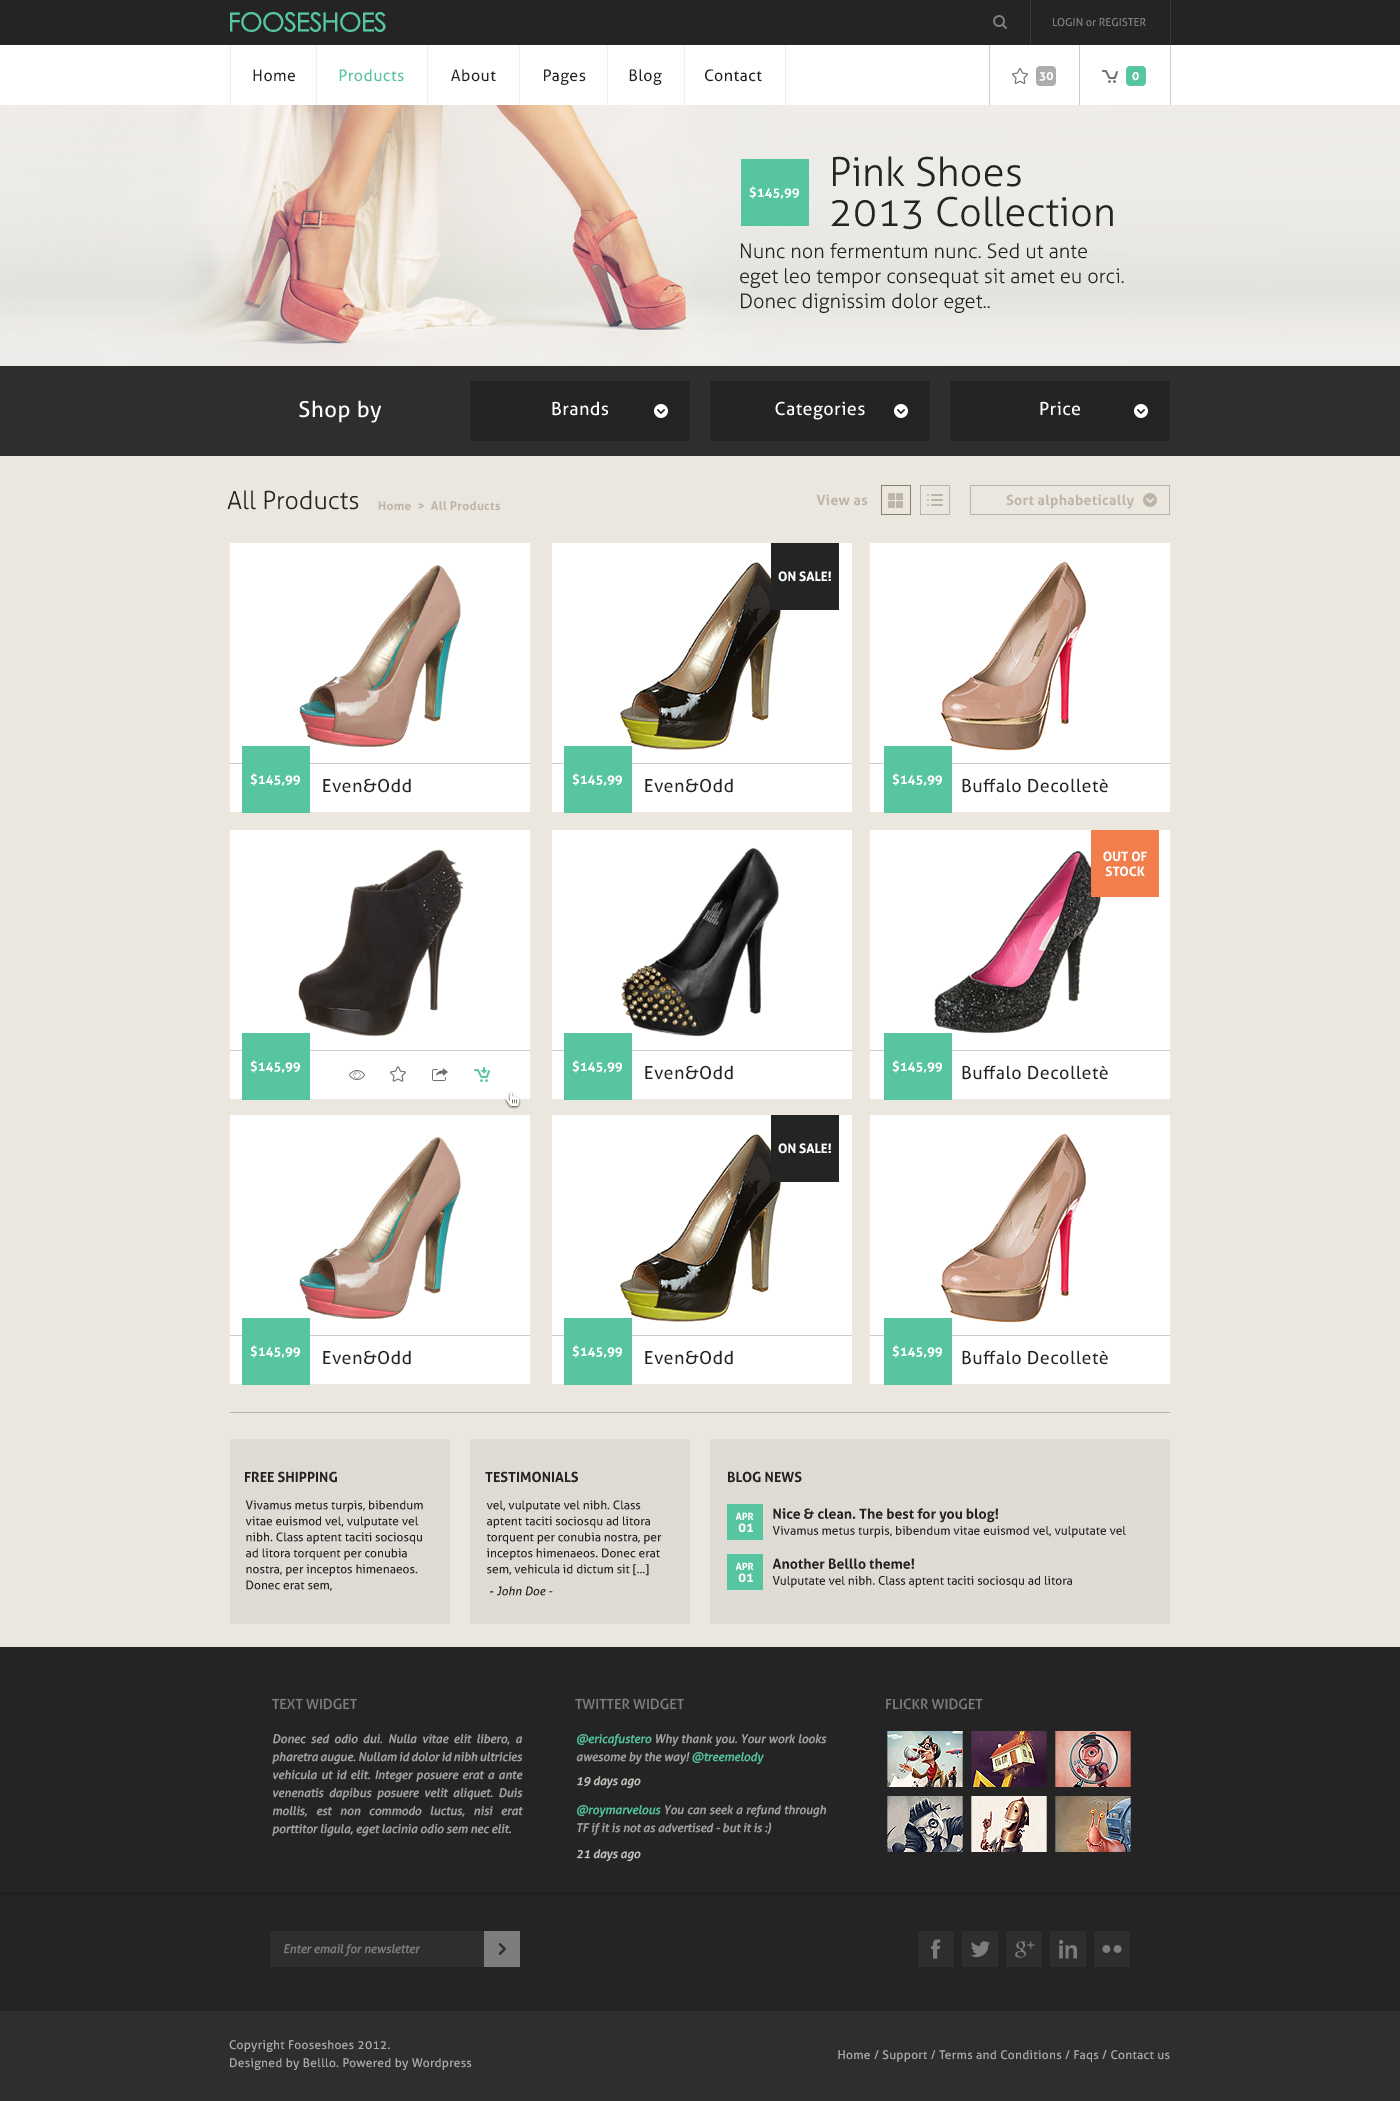
\includegraphics[width=0.4\textwidth]{demo.jpg}
    \caption{The best ecommerce UI in 2019}
\end{figure}

\blindtext

\blindtext

\blindtext

\begin{wrapfigure}{r}{3in}
\centering
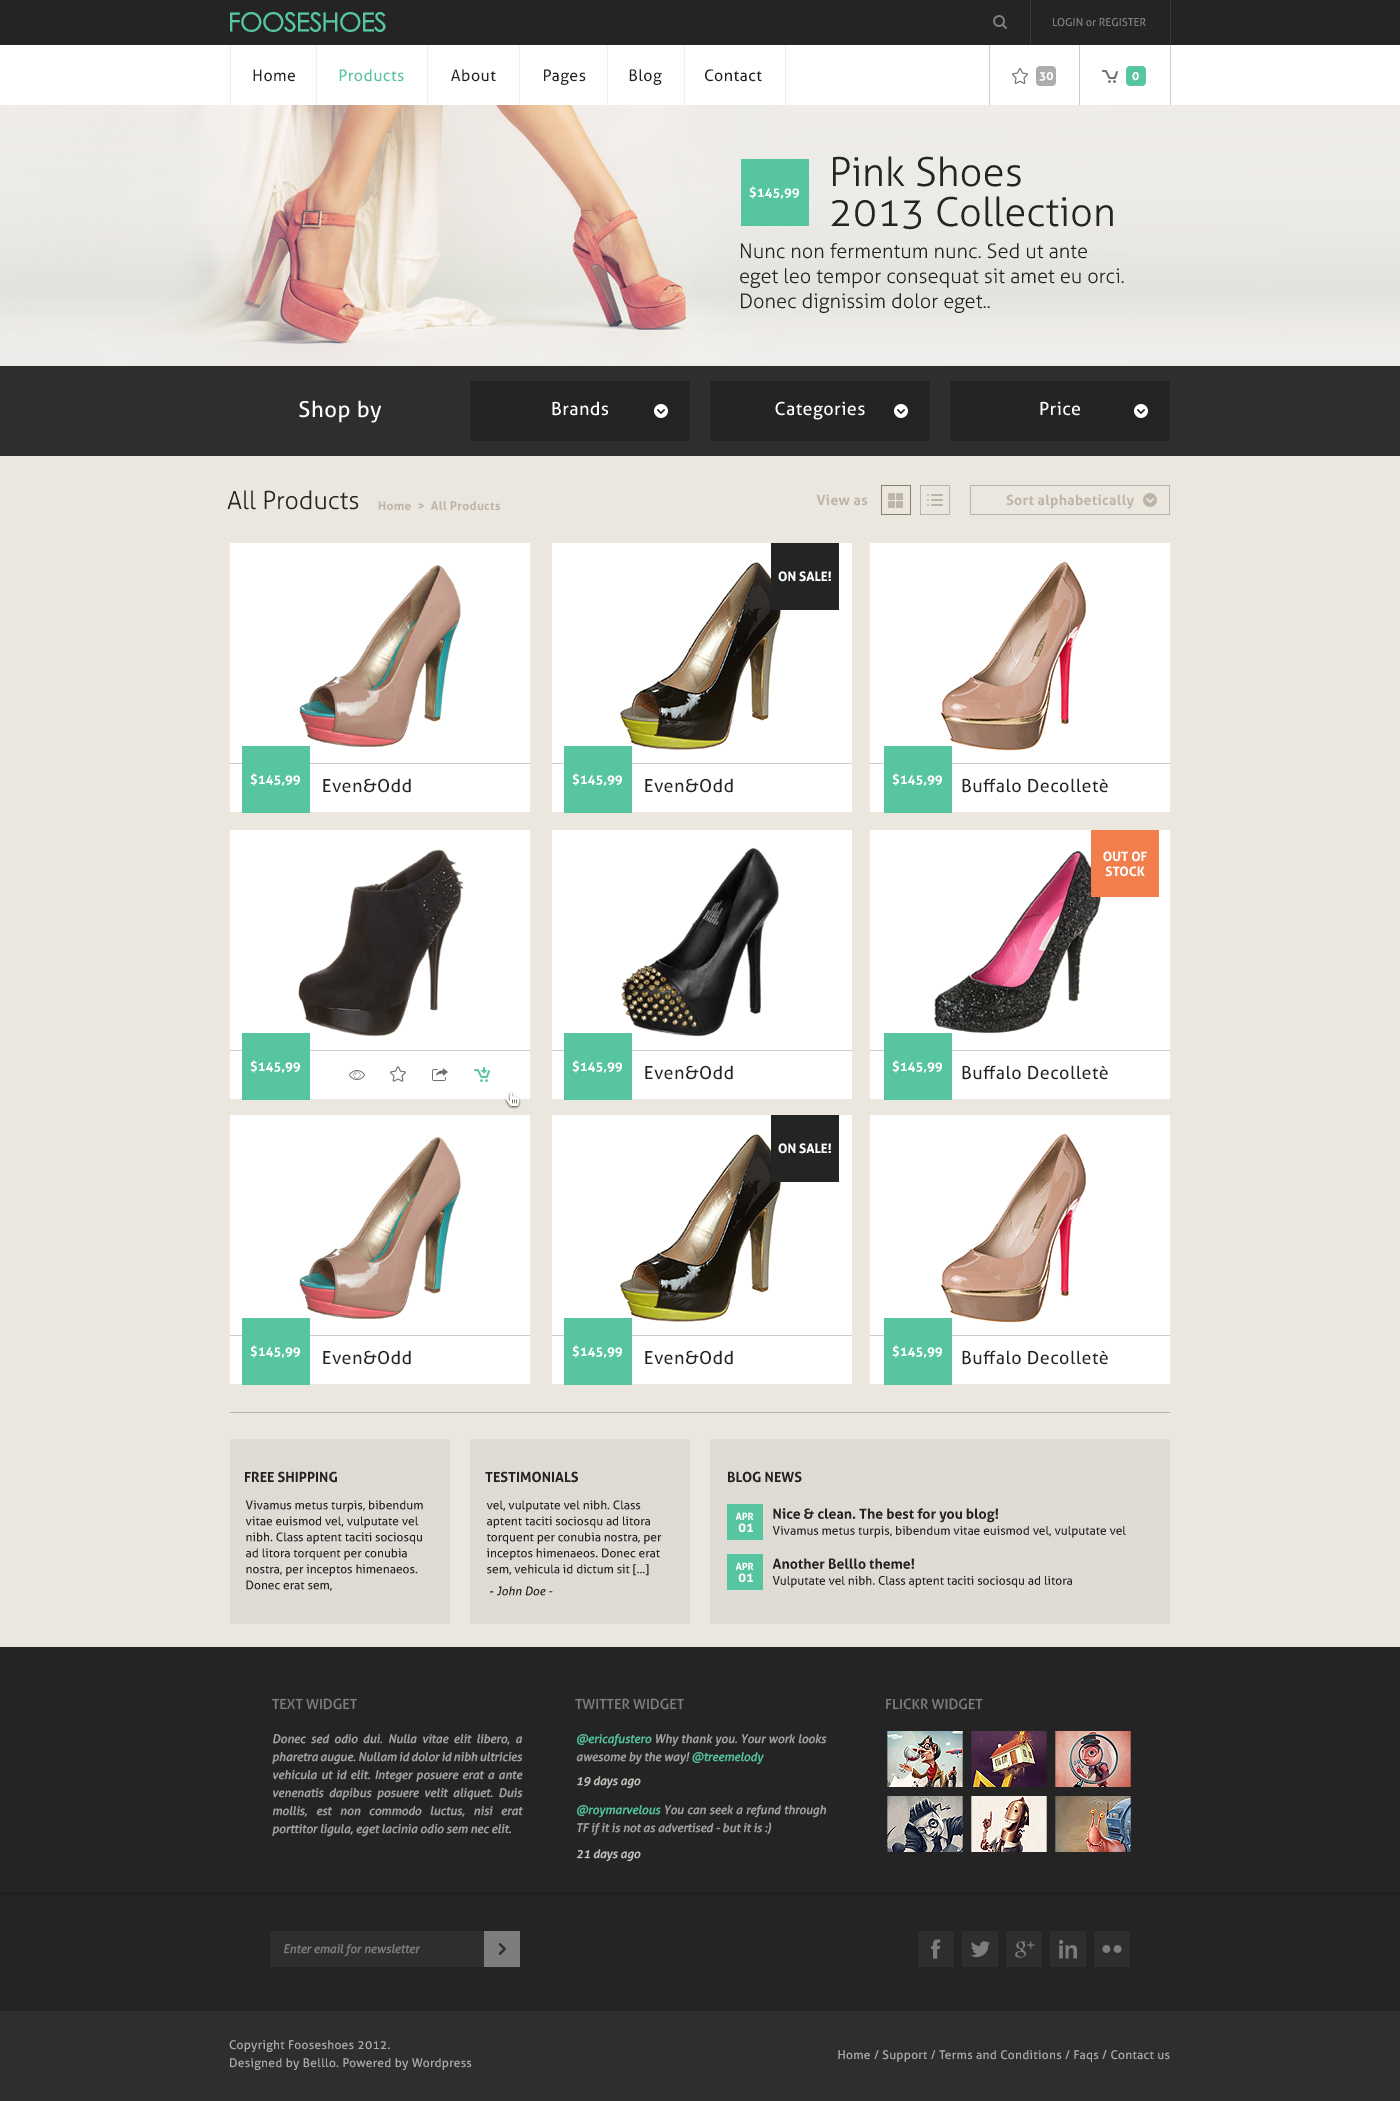
\includegraphics[width=1.5in, angle=90]{demo.jpg}
    \caption{The best ecommerce UI in 2019\label{latexpic}}
\end{wrapfigure}


\blindtext

\blindtext

\blindtext

\blindtext

\end{document}
